%%%%%%%% ICML 2026 EXAMPLE LATEX SUBMISSION FILE %%%%%%%%%%%%%%%%%

\documentclass{article}

% Recommended, but optional, packages for figures and better typesetting:
\usepackage{microtype}
\usepackage{graphicx}
\usepackage{subcaption}
\usepackage{booktabs} % for professional tables
\usepackage[normalem]{ulem}
\usepackage{amsmath}
\usepackage[makeroom]{cancel}

\usepackage{tikz}
\usetikzlibrary{arrows.meta, positioning, shapes.geometric, fit, backgrounds, calc}

% hyperref makes hyperlinks in the resulting PDF.
% If your build breaks (sometimes temporarily if a hyperlink spans a page)
% please comment out the following usepackage line and replace
% \usepackage{icml2026} with \usepackage[nohyperref]{icml2026} above.
\usepackage{hyperref}


% Attempt to make hyperref and algorithmic work together better:
\newcommand{\theHalgorithm}{\arabic{algorithm}}

% Use the following line for the initial blind version submitted for review:
\usepackage{icml2026}

% For preprint, use
% \usepackage[preprint]{icml2026}

% If accepted, instead use the following line for the camera-ready submission:
% \usepackage[accepted]{icml2026}

\usepackage{amsmath}
\usepackage{amssymb}
\usepackage{mathtools}
\usepackage{amsthm}


% if you use cleveref..
\usepackage[capitalize,noabbrev]{cleveref}

%%%%%%%%%%%%%%%%%%%%%%%%%%%%%%%%
% THEOREMS
%%%%%%%%%%%%%%%%%%%%%%%%%%%%%%%%
\theoremstyle{plain}
\newtheorem{theorem}{Theorem}[section]
\newtheorem{proposition}[theorem]{Proposition}
\newtheorem{lemma}[theorem]{Lemma}
\newtheorem{corollary}[theorem]{Corollary}
\theoremstyle{definition}
\newtheorem{definition}[theorem]{Definition}
\newtheorem{assumption}[theorem]{Assumption}
\theoremstyle{remark}
\newtheorem{remark}[theorem]{Remark}

% Todonotes is useful during development; simply uncomment the next line
%    and comment out the line below the next line to turn off comments
%\usepackage[disable,textsize=tiny]{todonotes}
\usepackage[textsize=tiny]{todonotes}

% The \icmltitle you define below is probably too long as a header.
% Therefore, a short form for the running title is supplied here:
\icmltitlerunning{Submission and Formatting Instructions for ICML 2026}

% \usepackage[margin=0.75in]{geometry}
\usepackage{tikz}
\usetikzlibrary{arrows.meta, positioning}
\usepackage{xcolor}
\usepackage{lipsum}

\definecolor{progblue}{RGB}{41, 98, 168}
\definecolor{fullred}{RGB}{192, 57, 43}
\definecolor{successgreen}{RGB}{39, 174, 96}
\definecolor{failgray}{RGB}{127, 140, 141}


\begin{document}

\twocolumn[
  \icmltitle{Progressive Cramming: Reliable Token Compression and What It Reveals}

  % It is OKAY to include author information, even for blind submissions: the
  % style file will automatically remove it for you unless you've provided
  % the [accepted] option to the icml2026 package.

  % List of affiliations: The first argument should be a (short) identifier you
  % will use later to specify author affiliations Academic affiliations
  % should list Department, University, City, Region, Country Industry
  % affiliations should list Company, City, Region, Country

  % You can specify symbols, otherwise they are numbered in order. Ideally, you
  % should not use this facility. Affiliations will be numbered in order of
  % appearance and this is the preferred way.
  \icmlsetsymbol{equal}{*}

  \begin{icmlauthorlist}
    \icmlauthor{Firstname1 Lastname1}{equal,yyy}
    \icmlauthor{Firstname2 Lastname2}{equal,yyy,comp}
    \icmlauthor{Firstname3 Lastname3}{comp}
    \icmlauthor{Firstname4 Lastname4}{sch}
    \icmlauthor{Firstname5 Lastname5}{yyy}
    \icmlauthor{Firstname6 Lastname6}{sch,yyy,comp}
    \icmlauthor{Firstname7 Lastname7}{comp}
    %\icmlauthor{}{sch}
    \icmlauthor{Firstname8 Lastname8}{sch}
    \icmlauthor{Firstname8 Lastname8}{yyy,comp}
    %\icmlauthor{}{sch}
    %\icmlauthor{}{sch}
  \end{icmlauthorlist}

  \icmlaffiliation{yyy}{Department of XXX, University of YYY, Location, Country}
  \icmlaffiliation{comp}{Company Name, Location, Country}
  \icmlaffiliation{sch}{School of ZZZ, Institute of WWW, Location, Country}

  \icmlcorrespondingauthor{Firstname1 Lastname1}{first1.last1@xxx.edu}
  \icmlcorrespondingauthor{Firstname2 Lastname2}{first2.last2@www.uk}

  % You may provide any keywords that you find helpful for describing your
  % paper; these are used to populate the "keywords" metadata in the PDF but
  % will not be shown in the document
  \icmlkeywords{Machine Learning, ICML}

  \vskip 0.3in
]

% this must go after the closing bracket ] following \twocolumn[ ...

% This command actually creates the footnote in the first column listing the
% affiliations and the copyright notice. The command takes one argument, which
% is text to display at the start of the footnote. The \icmlEqualContribution
% command is standard text for equal contribution. Remove it (just {}) if you
% do not need this facility.

% Use ONE of the following lines. DO NOT remove the command.
% If you have no special notice, KEEP empty braces:
\printAffiliationsAndNotice{}  % no special notice (required even if empty)
% Or, if applicable, use the standard equal contribution text:
% \printAffiliationsAndNotice{\icmlEqualContribution}

\begin{abstract}
    Token cramming compresses sequences into learned embeddings with near-perfect reconstruction, but prior work used fixed token budgets and 99\% accuracy thresholds, obscuring whether residual errors reflect optimization failures or fundamental limits.
    We introduce progressive cramming, which grows the target prefix token-by-token and stops only when reconstruction is no longer achievable within a fixed optimization budget.
    We further stabilize optimization with activation alignment and low-dimensional projection, enabling reliable 100\% reconstruction and more precise measurement of information gain.
    Using progressive trajectories, we find that optimization paths occupy surprisingly low-dimensional structure in the embedding space.
    Attention analysis shows that compression embeddings often become attention sinks in specific intermediate layers, which correlates with both optimization difficulty and downstream degradation.
    On likelihood-based multiple-choice evaluation (HellaSwag, ARC-Easy), prepending a perfectly reconstructing compression embedding reduces accuracy to close to random guessing across model families, even when the original prefix remains in context.
    Cramming achieves reconstruction by overriding model
    computation, not by encoding transferable semantics.
    Our results establish progressive cramming as a tool for
    studying compression limits while demonstrating that even
    perfect reconstruction is insufficient for meaningful
    compression.
\end{abstract}


\begin{figure}[h]
    \centering
    \input{visual_abstract.tikz}
    \caption{Full cramming achieves ${\sim}$1\% training error with teacher forcing, but errors cascade to 0\% generation accuracy. Progressive cramming establishes a precise boundary where compression either succeeds completely or fails clearly.}
    \label{fig:visual_abstract}
\end{figure}



% TODO выкидываем это в апендикс или основной текст?
% НЕ Уточнили границы крамминга
% А научились точно вовремя останавливать крамминг с идеальной точностью. А 1% ошибок - это очень плохо.


\section{Introduction}
\label{sec:introduction}

How much information can a single embedding encode?
Recent work on ``cramming'' \cite{kuratov2025cramming} probed this question by optimizing embeddings to reconstruct token sequences through autoregressive decoding.
The results were striking: single embeddings in the input space of large language models can encode up to 1568  tokens with near-perfect reconstruction accuracy, suggesting enormous latent capacity in transformer representations.

% PARAGRAPH 2: The open question - HOW does it work?
But \emph{how} do transformers achieve this?
The original work focused on capacity limits -- how many tokens fit -- rather than the mechanism enabling reconstruction.
This leaves open a fundamental question: does cramming discover dense semantic representations that the model can interpret, or does it exploit some other property of transformer computation?
Understanding this mechanism matters beyond cramming itself; it reveals how transformers process information stored in their embedding space.

% PARAGRAPH 3: Methodological improvements enabling study
We first address methodological limitations that complicate controlled study.
Prior work used fixed token budgets and 99\% accuracy thresholds with teacher forcing. But the last 1\% of errors may lead to catastrophic failures in autoregressive generation without teacher forcing.
We introduce \emph{progressive cramming}: sequentially adding tokens until perfect reconstruction, with two stabilizing techniques -- activation alignment and low-dimensional projection.
This achieves reliable 100\% accuracy and enables precise measurement of where compression fails. Figure~\ref{fig:visual_abstract} shows comparison of full and progressive cramming frameworks.

% PARAGRAPH 4: What we find - the mechanism
With these tools, we investigate the cramming mechanism.
Analysis of optimization trajectories reveals they occupy surprisingly low-dimensional manifolds: 30-100 PCA components explain 99\% of variance in 2048-4096 dimensional embedding spaces.
More critically, attention pattern analysis exposes \emph{how} reconstruction occurs: compression embeddings hijack 20-60\% of attention mass in intermediate layers.
We use the term \emph{attention hijacking} to emphasize that this attention concentration is associated with a breakdown of downstream language modeling capabilities, rather than benign attention focusing.
This concentration is invariant to sequence length -- the same layers are dominated whether cramming 32 or 512 tokens -- suggesting compression activates fixed circuits rather than scaling information density.

% PARAGRAPH 5: What this means - not semantic encoding
This mechanism has consequences.
If cramming worked through semantic encoding, compressed prefixes should preserve downstream capabilities.
Evaluation on HellaSwag and ARC reveals the opposite: models fail entirely, even when decompressed tokens remain in context.
Cramming achieves reconstruction by \emph{overriding} transformer computation -- forcing specific outputs through attention capture -- rather than by encoding information the model can flexibly use.

% PARAGRAPH 6: Implications
These findings reframe what cramming reveals about transformers.
The high capacity demonstrated by prior work reflects not dense semantic encoding but the ease of hijacking attention mechanisms.
This distinction matters for future work on learned compression: methods that override computation can achieve perfect reconstruction while encoding nothing transferable.

Our main contributions are as follows:
\begin{itemize}
    \item We introduce progressive cramming, which grows the target prefix token-by-token and targets 100\% reconstruction, enabling a sharp success/failure boundary beyond fixed-budget, 99\% protocols.
    \item We show that progressive optimization trajectories $\{\mathbf{e}^{(k)}\}$ are low-dimensional: across model families, 30--100 PCA components explain 99\% of per-sample trajectory variance in 2048--4096 dimensional embedding spaces.
    \item We quantify attention hijacking during cramming via attention mass to position 0 and find that compression embeddings can capture substantial mass in specific intermediate layers (often 20--60\%), with strong model-family dependence.
    \item We demonstrate that perfect reconstruction does not imply preserved downstream utility: on likelihood-based multiple-choice evaluation (HellaSwag, ARC-Easy), prepending a perfectly reconstructing compression embedding reduces accuracy to close to random guessing across model families, even when the original prefix remains in context.
\end{itemize}



% =============================================================================
\section{Related Work}
\label{sec:related_work}
% =============================================================================


\subsection{Token Cramming}

Our work is primarily built upon the token cramming framework introduced by \citet{kuratov2025cramming}, who demonstrates that per-sample optimization can compress up to 1,568 tokens into a single input embedding of Llama-3.1-8B, achieving compression ratios of approximately $1500\times$ -- two orders of magnitude beyond encoder-based approaches that typically achieve at most $10\times$ lossless compression. Their work reveals a substantial gap between the theoretical information capacity of high-dimensional embedding spaces and what current methods practically achieve. Crucially, they show that compression capacity is determined primarily by the cross-entropy reduction rather than raw sequence length, suggesting that the model leverages its internalized knowledge to complement the information stored in the embedding.

Extending this line of inquiry, \citet{mezentsev2025exploring} investigate whether autoregressive decoding is essential for reconstruction from compressed embeddings. They demonstrate that frozen LLMs can generate hundreds of accurate tokens in a single forward pass in non-autoregressive way when provided with just two learned ``proto-token'' embeddings, revealing an underexplored multi-token generation capability. Their analysis shows that valid compression representations form connected, local regions in embedding space rather than isolated points, suggesting the potential for learning practical encoders.


\subsection{Context Compression and Distillation}

A parallel line of research addresses context compression for the purpose of reducing computational costs during inference. Importantly, these approaches differ fundamentally from token cramming in their objective: they focus on \emph{semantic compression} that preserves task-relevant information for downstream use, rather than \emph{exact reconstruction} of the original token sequence.

\citet{zhang2025activations_beacon} propose Activation Beacon, a plug-in module that compresses the keys and values at every transformer layer into special beacon tokens. By directly compressing activations rather than relying on soft prompts to relay information, their method achieves flexible compression ratios while preserving the LLM's capabilities on short contexts. The progressive, chunk-wise compression workflow enables processing of contexts up to 400K tokens.

\citet{chevalier-etal-2023-autocompressors} adapt pre-trained language models into AutoCompressors that learn to compress long contexts into compact summary vectors through an unsupervised objective. These summary vectors function as soft prompts, enabling the model to condition on compressed representations of previous segments during language modeling. Their approach processes documents in segments, accumulating summary information across the sequence.

The In-Context Autoencoder (ICAE) \cite{ge2024ICAE} employs a LoRA-adapted encoder to compress contexts into memory slots that the target LLM can condition upon. Pre-trained with both autoencoding and language modeling objectives, ICAE achieves $4\times$ context compression while maintaining the ability to respond to various prompts. The method draws interesting parallels between working memory in cognitive science and context representation in LLMs.

These semantic compression methods are designed to preserve information relevant for downstream tasks such as question answering or summarization, tolerating lossy compression of details not essential for the target application. In contrast, our work and the cramming literature focus on near-lossless reconstruction, which provides a cleaner setting for studying the fundamental capacity and mechanisms of embedding-based information storage.

\subsection{Soft Prompts and Prefix Tuning}

The optimization of continuous embeddings as model inputs originated in parameter-efficient fine-tuning research. \citet{li-liang-2021-prefix-tuning} introduce prefix-tuning, which prepends learnable continuous vectors to the input that subsequent tokens can attend to as ``virtual tokens.'' By optimizing only $0.1\%$ of parameters while keeping the language model frozen, prefix-tuning achieves comparable performance to full fine-tuning on generation tasks while enabling efficient multi-task deployment.

\citet{lester-etal-2021-prompt-tuning} propose prompt tuning, a simplified approach that learns soft prompts only at the input layer rather than at every transformer layer. They demonstrate that prompt tuning becomes increasingly competitive with full model tuning as model scale increases, with billion-parameter models closing the gap entirely. This finding suggests that larger models develop embedding spaces with sufficient structure to support rich task-specific conditioning through input manipulation alone.

These methods establish that frozen language models can be effectively steered through learned embeddings without modifying model parameters. Token cramming can be viewed as an extreme case of this paradigm: rather than encoding task-specific instructions, the learned embedding must encode the complete information content of an arbitrary token sequence. Our progressive cramming methodology bridges these perspectives by studying how compression tokens interact with the model's attention and activation patterns as the encoding task becomes increasingly demanding.

% \paragraph{Mechanistic Interpretability.}
% {\color{red} TODO? Logit lens, activation patching, attention analysis. Methods we use for understanding hijacking.}


% =============================================================================
\section{Background: Token Cramming}
\label{sec:background}
% =============================================================================

\subsection{Problem Formulation}

In the cramming task, a single embedding is optimized to encode as many tokens as possible through autoregressive reconstruction. The language model weights remain frozen throughout optimization, and each sequence receives a newly initialized compression embedding.

Let $\mathcal{M}$ be an autoregressive language model with vocabulary $\mathcal{V}$ and embedding dimension $d$.
Given a target sequence $\mathbf{x} = (x_1, \ldots, x_n)$ where $x_i \in \mathcal{V}$, the cramming objective finds an embedding $\mathbf{e} \in \mathbb{R}^d$ such that:
%
\begin{equation}
    \mathbf{e}^* = \arg\min_{\mathbf{e}} \mathcal{L}_{\text{cram}}(\mathbf{e}; \mathbf{x}, \mathcal{M})
\end{equation}
%
where the cramming loss is the cross-entropy over the target sequence:
%
\begin{equation}
    \mathcal{L}_{\text{cram}}(\mathbf{e}; \mathbf{x}, \mathcal{M}) = -\sum_{i=1}^{n} \log p_{\mathcal{M}}(x_i \mid \mathbf{e}, x_1, \ldots, x_{i-1})
\end{equation}

\subsection{Limitations of Prior Work}\label{sec:prior_limitations}

Prior work on prompt compression and reconstruction typically evaluates success
using a fixed convergence threshold (e.g., 99\% token-level accuracy) under a
predefined token budget.
While convenient, this protocol obscures several important failure modes.

\paragraph{The 99\% threshold and the ``last 1\%'' problem.}
A 99\% reconstruction threshold implicitly treats the remaining 1\% of tokens as
negligible.
However, in autoregressive decoding, even a single early mismatch can cascade and
lead to complete divergence in subsequent generations.
Empirically, we observe that reconstruction errors are highly concentrated at the
earliest token positions.
As shown in Table~\ref{tab:compression_reconstruction_summary}, mismatches almost
exclusively occur at token indices 0 and 1, while later positions are typically reconstructed perfectly under teacher forcing.
This concentration indicates that the ``last 1\%'' of errors is not uniformly
distributed noise, but instead corresponds to structurally critical failures that
dominate downstream behavior.

\paragraph{Early-token brittleness under full cramming.}
The prevalence of mismatches at the first two tokens suggests a brittle regime in
which compression appears successful under teacher forcing, yet fails under greedy
generation.
Such early errors are especially problematic: once the autoregressive process
deviates from the target prefix, subsequent tokens are conditioned on an incorrect
history, rendering later reconstruction accuracy largely irrelevant.

\paragraph{Fixed token budgets obscure information-theoretic limits.}
Finally, evaluating reconstruction under a fixed token budget masks the true
capacity limits of compression.
A method may appear competitive simply because it saturates the allotted budget,
not because it approaches the minimal description length of the input.
By contrast, progressive cramming reveals how reconstruction quality degrades as
token budgets are varied, exposing trade-offs between compression rate, early-token
stability, and downstream generation fidelity.
The summary statistics in Table~\ref{tab:compression_reconstruction_summary}
highlight that comparable final convergence values can correspond to qualitatively
different mismatch profiles, underscoring the limitations of budget-constrained
evaluation protocols.


% =============================================================================
\section{Method: Progressive Cramming}
\label{sec:method}
% =============================================================================

\subsection{Progressive Token Addition}
\label{sec:progressive}

Rather than optimizing a compression embedding for a fixed-length target, we progressively extend the target prefix and warm-start optimization:
%
\begin{enumerate}
    \item Initialize with $\mathbf{x}^{(1)} = (x_1)$ and optimize $\mathbf{e}^{(1)} \in \mathbb{R}^d$ until perfect reconstruction.
    \item Extend to $\mathbf{x}^{(k)} = (x_1, \ldots, x_k)$, initialize $\mathbf{e}^{(k)} \leftarrow \mathbf{e}^{(k-1)}$, and continue optimizing for the longer prefix.
    \item Repeat until perfect reconstruction is no longer achievable within the optimization budget.
\end{enumerate}

This process is visualized on Figure~\ref{fig:progressive}.

Progressive cramming produces a sequence of embeddings $\{\mathbf{e}^{(k)}\}_{k=1}^{n}$, where $\mathbf{e}^{(k)}$ is the optimized compression embedding for the length-$k$ prefix.
This lets us quantify how far the optimizer moves in embedding space as new tokens are added.
We define the (stage-wise) trajectory length as the sum of Euclidean distances between consecutive stages:

\begin{equation}
    L_{\text{traj}} = \sum_{k=1}^{n-1} \left\| \mathbf{e}^{(k+1)} - \mathbf{e}^{(k)} \right\|_2
\end{equation}



\begin{figure}[t]
    \centering
    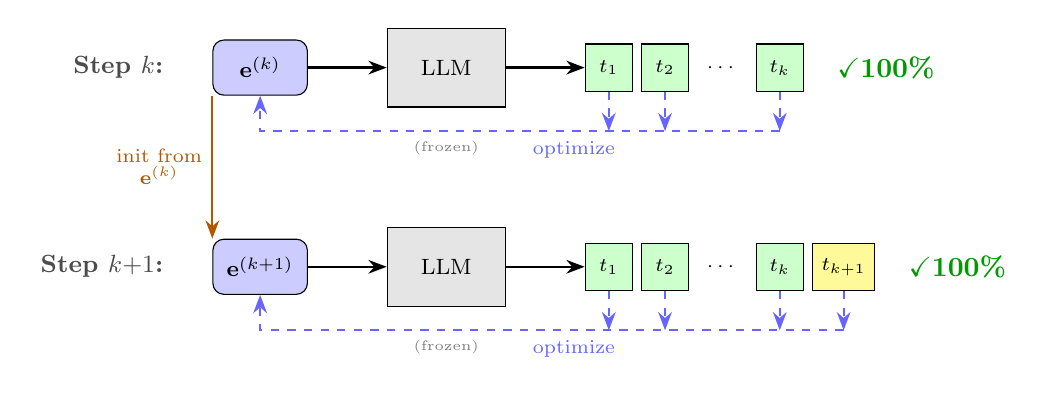
\begin{tikzpicture}[
    >=Stealth,
    node distance=0.8cm,
    emb/.style={draw, rounded corners, fill=blue!20, minimum width=1.2cm, minimum height=0.7cm, font=\footnotesize},
    llm/.style={draw, fill=gray!20, minimum width=1.5cm, minimum height=1cm, font=\footnotesize},
    token/.style={draw, fill=green!20, minimum width=0.6cm, minimum height=0.6cm, font=\scriptsize},
    check/.style={text=green!60!black, font=\bfseries},
    stage/.style={font=\small\bfseries, text=black!70},
    optim/.style={->, thick, blue!60, dashed},
    init/.style={->, thick, orange!70!black},
]

% === STAGE k ===
\node[stage] (stage1) {\makebox[1.5cm][r]{Step $k$}:};

\node[emb, right=0.5cm of stage1] (e1) {$\mathbf{e}^{(k)}$};
\node[llm, right=1cm of e1] (llm1) {LLM};
\node[token, right=1cm of llm1] (t1_1) {$t_1$};
\node[token, right=0.1cm of t1_1] (t1_2) {$t_2$};
\node[right=0.1cm of t1_2, font=\scriptsize] (dots1) {$\cdots$};
\node[token, right=0.1cm of dots1] (t1_k) {$t_k$};

% Arrows for stage k
\draw[->, thick] (e1) -- (llm1);
\draw[->, thick] (llm1) -- (t1_1);

% Checkmark
\node[check, right=0.3cm of t1_k] (check1) {\checkmark 100\%};

% Optimization loop for stage k - spans all tokens
\coordinate (loop1_right) at ($(t1_k.south) + (0, -0.5)$);
\coordinate (loop1_left) at ($(t1_1.south) + (0, -0.5)$);
\draw[optim] (t1_1.south) -- (loop1_left);
\draw[optim] (t1_2.south) -- ++(0, -0.5);
\draw[optim] (t1_k.south) -- (loop1_right);
\draw[optim] (loop1_right) -- (loop1_left) -| node[pos=0.05, below, font=\scriptsize, text=blue!60] {optimize} (e1.south);

% === STAGE k+1 ===
\node[stage, below=2cm of stage1] (stage2) {\makebox[1.5cm][r]{Step $k{+}1$}:};

\node[emb, right=0.5cm of stage2] (e2) {$\mathbf{e}^{(k+1)}$};
\node[llm, right=1cm of e2] (llm2) {LLM};
\node[token, right=1cm of llm2] (t2_1) {$t_1$};
\node[token, right=0.1cm of t2_1] (t2_2) {$t_2$};
\node[right=0.1cm of t2_2, font=\scriptsize] (dots2) {$\cdots$};
\node[token, right=0.1cm of dots2] (t2_k) {$t_k$};
\node[token, right=0.1cm of t2_k, fill=yellow!40] (t2_k1) {$t_{k+1}$};

% Arrows for stage k+1
\draw[->, thick] (e2) -- (llm2);
\draw[->, thick] (llm2) -- (t2_1);

% Checkmark
\node[check, right=0.3cm of t2_k1] (check2) {\checkmark 100\%};

% Optimization loop for stage k+1 - spans all tokens
\coordinate (loop2_right) at ($(t2_k1.south) + (0, -0.5)$);
\coordinate (loop2_left) at ($(t2_1.south) + (0, -0.5)$);
\draw[optim] (t2_1.south) -- (loop2_left);
\draw[optim] (t2_2.south) -- ++(0, -0.5);
\draw[optim] (t2_k.south) -- ++(0, -0.5);
\draw[optim] (t2_k1.south) -- (loop2_right);
\draw[optim] (loop2_right) -- (loop2_left) -| node[pos=0.05, below, font=\scriptsize, text=blue!60] {optimize} (e2.south);

% === INITIALIZATION ARROW ===
\draw[init] (e1.south west) -- (e2.north west)
    node[midway, left, font=\scriptsize, text=orange!70!black, align=center] {init from\\$\mathbf{e}^{(k)}$};

% === LABELS ===
\node[below=0.3cm of llm1, font=\tiny, text=gray] {(frozen)};
\node[below=0.3cm of llm2, font=\tiny, text=gray] {(frozen)};

\end{tikzpicture}
    \caption{Progressive cramming adds target tokens sequentially. At stage $k$, we optimize the compression representation to achieve 100\% reconstruction of the prefix $(x_1,\ldots,x_k)$, then extend to $k{+}1$ and warm-start from the previous solution.}
    \label{fig:progressive}
\end{figure}

\subsection{Activation Alignment}
\label{sec:activation_alignment}

To stabilize optimization, we regularize hidden states toward those of the uncompressed sequence.
Let $\mathbf{h}_l^{\text{cram}}(i)$ denote the hidden state at layer $l$ and token position $i$ when the model is conditioned on the compression embedding, and let $\mathbf{h}_l^{\text{clean}}(i)$ be the corresponding state for the same token position without compression.
We align activations using cosine distance:
%
\begin{equation}
    \mathcal{L}_{\text{align}} = \frac{1}{n} \sum_{l=1}^{K} \sum_{i=1}^{n} \left( 1 - \frac{\mathbf{h}_l^{\text{cram}}(i) \cdot \mathbf{h}_l^{\text{clean}}(i)}{\|\mathbf{h}_l^{\text{cram}}(i)\| \, \|\mathbf{h}_l^{\text{clean}}(i)\|} \right)
\end{equation}
%

where $K$ is the number of layers used for alignment. We align the first $K$ transformer layers (closest to the embedding layer).

The full objective combines reconstruction and alignment:

\begin{equation}
    \mathcal{L} = \mathcal{L}_{\text{cram}} + \alpha \mathcal{L}_{\text{align}}
\end{equation}

where $\alpha$ controls alignment strength.


\subsection{Low-Dimensional Projection}
\label{sec:lowdim}

We observed that optimization trajectories occupy low-dimensional subspaces (Section~\ref{sec:trajectory}).
This motivates constraining optimization to a learned projection:

\begin{equation}
    \mathbf{e} = \mathbf{W} \mathbf{z} + \mathbf{b}
\end{equation}

where $\mathbf{z} \in \mathbb{R}^k$ with $k \ll d$, $\mathbf{W} \in \mathbb{R}^{d \times k}$, and $\mathbf{b} \in \mathbb{R}^d$.
For each sample, we randomly initialize $(\mathbf{W}, \mathbf{b}, \mathbf{z})$ and optimize them jointly, which restricts the compression embedding to a rank-$k$ affine subspace.

After optimization, the effective embedding $\mathbf{e}$ can be materialized once and reused; the projection primarily changes the optimization geometry by introducing optimizer state (e.g., momentum) in the low-dimensional coordinates.

\subsection{Attention Mass}
\label{sec:attention_mass}

To quantify attention hijacking (Section~\ref{sec:attention}), we measure how much attention mass other positions allocate to the first position (position $0$), which corresponds to the compression embedding in crammed inputs or the BOS token in the uncompressed baseline.
Let $\mathbf{A}_l \in [0,1]^{S \times S}$ denote the attention matrix at layer $l$ after averaging over heads.
For a given prefix length $s \le S$, we define the attention mass on position $0$ as
%
\begin{equation}
    m_l(s) = \frac{1}{s-1} \sum_{q=1}^{s-1} \mathbf{A}_l(q, 0)
\end{equation}
%
which excludes self-attention ($q=0$) and averages over query positions.
We report $100 \cdot m_l(s)$ as a percentage, and average over a set of target prefix lengths $\mathcal{S}$:
%
\begin{equation}
    \bar{m}_l = \frac{1}{|\mathcal{S}|} \sum_{s \in \mathcal{S}} m_l(s)
\end{equation}

\subsection{Information Gain}

As a primary cramming metric we use information gain \cite{kuratov2025cramming}, defined as the reduction in total cross-entropy (in bits) on the target sequence when conditioning on the learned compression embedding.
Let $H_{LM}$ be the sum of per-token cross-entropies for the original token sequence, and let $H_{\mathrm{comp}+LM}$ be the corresponding quantity when the model is conditioned on the compression embedding.

\begin{equation}
    C_H = H_{LM} - H_{\mathrm{comp}+LM}
\end{equation}

\citet{kuratov2025cramming} show that cramming capacity is better characterized by information gain than by raw token count, and that this quantity is relatively stable across datasets.

% =============================================================================
\section{Experiments}
\label{sec:experiments}
% =============================================================================

We evaluate progressive cramming on PG19 \cite{Rae2020CompressiveTransformerPG19} across four model families: Pythia \cite{biderman2023pythia}, Llama~3 \cite{dubey2024llama3}, SmolLM2 \cite{allal2025smollm2}, and Gemma~3 \cite{gemma3}.

Table~\ref{tab:full_vs_progressive} compares progressive cramming (targeting 100\% reconstruction) to ``full'' cramming baselines that use fixed token budgets and may terminate below perfect accuracy.
Because autoregressive decoding is brittle to early errors (Section~\ref{sec:prior_limitations}), we interpret this comparison primarily through the lens of \emph{perfect} reconstruction: progressive cramming trades a fixed-budget constraint for a fixed-accuracy constraint.
In the default setting, progressive cramming underperforms full cramming in both information gain and reconstructed length.
However, adding regularization via activation alignment and low-dimensional projection (Section~\ref{sec:activation_alignment_exp}) can recover capacity; for Llama-3.1-8B we reach $5103 \pm 748$ bits of information gain, comparable to $4865.7 \pm 546.6$ reported by \citet{kuratov2025cramming}.

\begin{table}[]
    \centering
    \caption{Full vs. progressive cramming on PG19 (mean $\pm$ std over samples). ``Full'' cramming uses a fixed token budget and may stop below perfect reconstruction \cite{kuratov2025cramming}; progressive cramming fixes reconstruction at 100\% and reports the achieved token count.}
    \label{tab:full_vs_progressive}

    \begin{tabular}{llll}
        \hline
         Type                                           & Tokens                  & Info Gain                & Accuracy                   \\
        \hline
         \multicolumn{4}{l}{\textbf{Llama-3.1-8B}} \\
         Full                                           & 1568                    & 5002 {\small $\pm$ 850}  & 0.997 {\small $\pm$ 0.003} \\
         Progr.                                         & 1064 {\small $\pm$ 394} & 3028 {\small $\pm$ 1321} & 1.0                        \\
         \midrule \midrule
         \multicolumn{4}{l}{\textbf{Pythia1.4b}} \\
         Full                                           & 256                     & 802 {\small $\pm$ 113}   & 0.985 {\small $\pm$ 0.031} \\
         Progr.                                         & 544 {\small $\pm$ 57}   & 1694 {\small $\pm$ 125}  & 1.0                        \\
        \hline
        \end{tabular}

\end{table}


\begin{table*}[]
    \centering
    \caption{Progressive cramming variants and key metrics across model families. For each family we report baseline progressive cramming, low-dimensional projection only (``dim''), activation alignment only ($\alpha$, $L$), and their combination.}
    \label{tab:all_progressive_modifications}

    \begin{tabular}{lllll}
        \hline
         Model                                                               & Compressed Tokens           & Information Gain         & Trajectory Length         & PCA 99\%                  \\
        \hline
         Llama-3.1-8B {\small lr=0.1}                                        & 1063.5 {\small $\pm$ 394.4} & 3028 {\small $\pm$ 1321} & 4861 {\small $\pm$ 1033}  & 74.4 {\small $\pm$ 7.94} \\
         Llama-3.1-8B {\small $\alpha=1.0$} {\small $L=8$}                   & 1633.3 {\small $\pm$ 275.4} & 5130 {\small $\pm$ 247}  & 1146 {\small $\pm$ 137}   & 40 {\small $\pm$ 1.26}   \\
         Llama-3.1-8B {\small dim=32}                                        & 1745 {\small $\pm$ 306}     & 5312 {\small $\pm$ 330}  & 10250 {\small $\pm$ 3256} & 35.7 {\small $\pm$ 5.1}  \\
         Llama-3.1-8B {\small dim=32} {\small $\alpha=1.0$} {\small $L=8$}   & 1804.8 {\small $\pm$ 297.8} & 5103 {\small $\pm$ 748}  & 13584 {\small $\pm$ 3823} & 34.7 {\small $\pm$ 5.37} \\
         \midrule
         pythia-1.4b {\small lr=0.5}                                         & 543.8 {\small $\pm$ 56.8}   & 1694 {\small $\pm$ 125}  & 6730 {\small $\pm$ 390}   & 49 {\small $\pm$ 3.32}   \\
         pythia-1.4b {\small $\alpha=1.0$} {\small $L=8$}                    & 178.7 {\small $\pm$ 33.1}   & 524 {\small $\pm$ 92}    & 80 {\small $\pm$ 13}      & 14.3 {\small $\pm$ 1.79} \\
         pythia-1.4b {\small dim=256}                                        & 375.5 {\small $\pm$ 100.7}  & 1189 {\small $\pm$ 314}  & 2135 {\small $\pm$ 1312}  & 16.5 {\small $\pm$ 2.16} \\
         pythia-1.4b {\small dim=256} {\small $\alpha=1.0$} {\small $L=8$}   & 498.2 {\small $\pm$ 92.7}   & 1555 {\small $\pm$ 146}  & 5396 {\small $\pm$ 3309}  & 19.6 {\small $\pm$ 5.89} \\
         \midrule
         SmolLM2-1.7B {\small lr=0.1}                                        & 370.2 {\small $\pm$ 113.1}  & 1119 {\small $\pm$ 350}  & 1027 {\small $\pm$ 167}   & 29.2 {\small $\pm$ 2.93} \\
         SmolLM2-1.7B {\small $\alpha=1.0$} {\small $L=4$}                   & 186.9 {\small $\pm$ 47.3}   & 530 {\small $\pm$ 104}   & 85 {\small $\pm$ 8}       & 13.3 {\small $\pm$ 1.73} \\
         SmolLM2-1.7B {\small dim=256}                                       & 487.7 {\small $\pm$ 152.7}  & 1449 {\small $\pm$ 402}  & 2265 {\small $\pm$ 1405}  & 16 {\small $\pm$ 4.47}   \\
         SmolLM2-1.7B {\small dim=256} {\small $\alpha=1.0$} {\small $L=8$}  & 468 {\small $\pm$ 243.7}    & 1350 {\small $\pm$ 621}  & 6544 {\small $\pm$ 9765}  & 11.6 {\small $\pm$ 3.61} \\
         \midrule
         gemma-3-4b-pt {\small lr=0.1}                                       & 286.5 {\small $\pm$ 164.6}  & 949 {\small $\pm$ 466}   & 1044 {\small $\pm$ 328}   & 31.8 {\small $\pm$ 9.21} \\
         gemma-3-4b-pt {\small $\alpha=1.0$} {\small $L=8$}                  & 75.1 {\small $\pm$ 84.9}    & 268 {\small $\pm$ 256}   & 65 {\small $\pm$ 44}      & 9.3 {\small $\pm$ 3.93}  \\
         gemma-3-4b-pt {\small dim=256}                                      & 252.7 {\small $\pm$ 189.9}  & 829 {\small $\pm$ 635}   & 1372 {\small $\pm$ 886}   & 13.1 {\small $\pm$ 4.83} \\
         gemma-3-4b-pt {\small dim=256} {\small $\alpha=1.0$} {\small $L=8$} & 217.1 {\small $\pm$ 146.2}  & 719 {\small $\pm$ 425}   & 1091 {\small $\pm$ 557}   & 13.3 {\small $\pm$ 2.69} \\
        \hline
    \end{tabular}

\end{table*}


\subsection{Optimization Trajectories}
\label{sec:trajectory}

Progressive cramming enables tracking the optimization path through embedding space.
We record the sequence of optimized embeddings $\{\mathbf{e}^{(k)}\}_{k=1}^{n}$ and analyze its geometry.
For each sample, we run PCA on the stage embeddings $\{\mathbf{e}^{(k)}\}_{k=1}^{n}$ across $k$ (using standard PCA mean-centering across stages) and define ``PCA 99\%'' as the minimum number of components whose cumulative explained-variance ratio reaches 99\%.
We report this quantity averaged over samples.
Across model families, trajectories are well-approximated by low-dimensional structure: a modest number of principal components explains 99\% of the trajectory variance, even when hundreds (or thousands) of tokens are reconstructed (Table~\ref{tab:all_progressive_modifications}).

Notably, Gemma~3 achieves lower information gain at shorter reconstructed lengths than Llama and Pythia, consistent with stronger architectural or training-time constraints (e.g., logits softcapping \cite{gemma2}).
One plausible mechanism is that logit softcapping limits the model's ability to produce extremely peaked next-token distributions. Since cramming optimization implicitly pushes the model toward high-confidence, token-specific predictions over long horizons, bounding logit magnitudes can reduce the maximum separability between the correct token and close alternatives and can damp gradients in the high-confidence regime. Both effects may make it harder to reach perfect autoregressive reconstruction with a fixed optimization budget, yielding lower information gain and earlier saturation in reconstructed length.

Figure~\ref{fig:visual_abstract_optimization_trajectory_with_good_accuracy} visualizes a single trajectory projected onto the first two principal components.
As the reconstructed prefix grows, the region of embeddings that attains near-perfect teacher-forced reconstruction contracts, suggesting that the optimization landscape becomes increasingly constrained at longer lengths.

Figure~\ref{fig:pca_from_seq_length} shows that for Llama-3.1-8B, the number of components required to explain 99\% variance grows sublinearly with prefix length and follows a slow (approximately logarithmic) trend across learning rates.


\begin{figure}[t]
    \centering
    \includegraphics[width=1.0\linewidth]{visual_abstract_pc1_pc2_joined.pdf}
    \caption{Progressive cramming trajectory for a length-1000 sequence on Llama3-8B, projected onto the first two PCA components. Each black point is the optimized compression embedding for a given prefix length. For prefix lengths \(\{100, 200, 400, 800, 1000\}\), we additionally visualize the local accuracy landscape in this 2D plane (color saturation indicates higher reconstruction accuracy, capped at 90\%). As sequence length increases, the basin of near-perfect reconstruction shrinks, making optimization harder. The first two PCA components explain 65.7\% of the trajectory variance.}
    \label{fig:visual_abstract_optimization_trajectory_with_good_accuracy}
\end{figure}


\begin{figure}[t]
    \centering
    \centerline{\includegraphics[width=\columnwidth]{aggregate_pca_components_vs_seq_len_Llama3.1-8B_all_lrs.pdf}}
    \caption{Number of principal components required to explain 99\% of progressive trajectory variance vs. reconstructed prefix length for Llama-3.1-8B, shown for multiple learning rates.}
    \label{fig:pca_from_seq_length}
\end{figure}


\subsection{Low-Dimensional Projection}

Low-dimensional projection (Section~\ref{sec:lowdim}) changes the optimization geometry by restricting the learned embedding to an affine rank-$k$ subspace.
Empirically, this can improve stability and alter the effective capacity:
\begin{itemize}
    \item It often reduces sensitivity to learning rate by concentrating optimization into a smaller coordinate system.
    \item It can reduce the intrinsic dimensionality of trajectories (PCA 99\%) while preserving, or sometimes increasing, information gain.
\end{itemize}

Table~\ref{tab:all_progressive_modifications} compares baseline progressive cramming to a representative low-dimensional projection setting (``dim'') for each family.
Two takeaways stand out:
\begin{itemize}
    \item For Llama-3.1-8B and SmolLM2-1.7B, projection can substantially increase achievable token counts and information gain compared to the unconstrained baseline.
    \item For Pythia-1.4B projection can reduce token count and information gain relative to the baseline; combining projection with activation alignment partially recovers performance compared to projection alone.
\end{itemize}


\subsection{PCA Reconstruction}
\label{sec:pca_reconstruction}

We evaluate reconstruction accuracy when progressive embeddings are reconstructed from PCA components.
Figure~\ref{fig:pca_reconstruction_accuracy} reports accuracy as a function of the number of components.
Although Table~\ref{tab:all_progressive_modifications} suggests that for Llama-3.1-8B roughly 74 PCA components explain 99\% of trajectory variance, achieving near-perfect teacher-forced reconstruction requires substantially more components.
We also observe the same failure mode as in the full cramming setup (Section~\ref{sec:prior_limitations}):
errors cluster at the start of the sequence (often at the first decoded token), which then propagates and breaks subsequent autoregressive decoding.
This behavior appears whenever reconstruction accuracy is below 100\%; with perfect reconstruction, this failure mode disappears.

\begin{figure}[t]
    \centering
    \centerline{\includegraphics[width=\columnwidth]{aggregate_pca_reconstruction_accuracy.pdf}}
    \caption{Teacher-forced reconstruction accuracy for PCA-reconstructed compression embeddings vs. number of PCA components (Llama-3.1-8B).}
    \label{fig:pca_reconstruction_accuracy}
\end{figure}

\subsection{Activation Alignment}
\label{sec:activation_alignment_exp}

Table~\ref{tab:all_progressive_modifications} studies activation alignment (defined in Section~\ref{sec:activation_alignment}) and its interaction with low-dimensional projection.
Alignment acts as a regularizer: it can significantly reduce trajectory length and PCA 99\% (indicating smoother, more constrained optimization), but it may trade off against raw cramming capacity depending on the model family.
In particular, for Llama-3.1-8B, alignment increases information gain and token count relative to the baseline, whereas for SmolLM2-1.7B and Pythia-1.4B alignment alone reduces capacity but can be combined with projection to recover part of the loss.
Across settings, we observe that alignment qualitatively changes attention behavior, often pushing attention hijacking effects toward deeper layers.


\subsection{Attention Hijacking}
\label{sec:attention}

Perfect reconstruction can arise from qualitatively different mechanisms, ranging from faithful information encoding to brittle steering that overrides the model's normal computation; to probe the mechanism, we analyze whether the compression embedding becomes an \emph{attention sink} that captures a disproportionate fraction of attention, analogous to (and potentially competing with) the BOS token.
We quantify this effect using the attention-mass metric from Section~\ref{sec:attention_mass}, comparing attention directed to position 0 in the crammed setting (compression embedding) against attention directed to position 0 in the uncompressed baseline (BOS).

Table~\ref{tab:attn_hijacking} shows that attention hijacking is highly model-dependent when aggregated over layers.
SmolLM2 and Pythia exhibit strong correlation between the layer-wise attention-mass profiles for the BOS token and the compression embedding.
In these families, the compression embedding attracts substantial attention mass in the same layers where BOS is an attention sink; in Pythia it can match or exceed BOS attention on average.
This suggests that the compression embedding may function as an attention sink, but one that can override the model's normal computation and degrade downstream behavior (Section~\ref{sec:semantic_evaluation}).

In contrast, Llama and Gemma show much lower compression-embedding attention mass than BOS on average and weak (or negative) correlation, suggesting that hijacking concentrates in specific layers rather than uniformly matching the BOS pattern.

Motivated by this similarity, we test whether including both a BOS token and a compression embedding in the prompt creates interference between two attention sinks.
We therefore run ablations that remove the BOS token and recompute progressive cramming metrics (Table~\ref{tab:progressive_no_bos_token}).
Removing BOS increases reconstructed length and information gain (and reduces compression-embedding attention mass) for Llama-3.1-8B, but has little effect on the other model families.

\begin{table*}[]
    \centering
    \caption{Attention hijacking summary. ``Compression Embedding'' is attention mass to position 0 for the compression embedding in the crammed input; ``BOS Token'' is attention mass to position 0 for the uncompressed baseline; ``Diff'' is (Compression$-$BOS). ``Correlation'' is the Pearson correlation between per-layer attention-mass profiles. \bcancel{B} stands for removed BOS token for cramming compression column.}
    \label{tab:attn_hijacking}


    \begin{tabular}{llllr}
    \hline
     Model                               & Compression Embedding (\%)  & BOS Token Original (\%)     & Diff (\%)                    &   Correlation \\
    \hline
     Llama-3.2-1B {\small lr=0.1}        & 20.71 {\small $\pm$ 5.74}  & 67.37 {\small $\pm$ 1.41}  & -46.66 {\small $\pm$ 6.5}   &        0.2884 \\
     Llama-3.2-3B {\small lr=0.1}        & 15.97 {\small $\pm$ 1.15}  & 70 {\small $\pm$ 1.14}     & -54.03 {\small $\pm$ 1.01}  &       -0.1907 \\
     Llama-3.1-8B {\small lr=0.1}        & 38.07 {\small $\pm$ 17.98} & 70.56 {\small $\pm$ 1.26}  & -32.49 {\small $\pm$ 18.96} &        0.4104 \\
     Llama-3.1-8B\ \bcancel{B} {\small lr=0.1}  & 18.93 {\small $\pm$ 10.43} & 70.05 {\small $\pm$ 1.29}  & -51.12 {\small $\pm$ 10.33} &        0.4688 \\
     \midrule
     pythia-160m {\small lr=0.5}         & 50.88 {\small $\pm$ 16.11} & 36.15 {\small $\pm$ 2.75}  & 14.72 {\small $\pm$ 15.65}  &        0.7877 \\
     pythia-410m {\small lr=0.5}         & 34.69 {\small $\pm$ 15.35} & 39.96 {\small $\pm$ 1.86}  & -5.27 {\small $\pm$ 15.63}  &        0.7883 \\
     pythia-1.4b {\small lr=0.5}         & 37.41 {\small $\pm$ 4.12}  & 24.03 {\small $\pm$ 2.49}  & 13.37 {\small $\pm$ 5.17}   &        0.8315 \\
     pythia-1.4b\ \bcancel{B} {\small lr=0.5}   & 38 {\small $\pm$ 4.72}     & 24.74 {\small $\pm$ 2.49}  & 13.27 {\small $\pm$ 5.89}   &        0.8454 \\
     \midrule
     SmolLM2-135M {\small lr=0.1}        & 60.79 {\small $\pm$ 17.6}  & 74.04 {\small $\pm$ 11.45} & -13.25 {\small $\pm$ 23.9}  &        0.8475 \\
     SmolLM2-360M {\small lr=0.1}        & 65.71 {\small $\pm$ 16.07} & 69.05 {\small $\pm$ 9.6}   & -3.34 {\small $\pm$ 19.42}  &        0.9843 \\
     SmolLM2-1.7B {\small lr=0.1}        & 49.85 {\small $\pm$ 2.75}  & 56.47 {\small $\pm$ 9.19}  & -6.62 {\small $\pm$ 9.32}   &        0.9532 \\
     SmolLM2-1.7B\ \bcancel{B} {\small lr=0.1}  & 49.95 {\small $\pm$ 2.82}  & 56.47 {\small $\pm$ 9.19}  & -6.52 {\small $\pm$ 9.44}   &        0.9535 \\
     \midrule
     gemma-3-270m {\small lr=0.1}        & 12.94 {\small $\pm$ 3.04}  & 60.87 {\small $\pm$ 1.43}  & -47.93 {\small $\pm$ 3.87}  &        0.3448 \\
     gemma-3-1b-pt {\small lr=0.1}       & 18.67 {\small $\pm$ 3.14}  & 61.27 {\small $\pm$ 1.73}  & -42.6 {\small $\pm$ 3.01}   &        0.0998 \\
     gemma-3-4b-pt {\small lr=0.1}       & 7.97 {\small $\pm$ 2.09}   & 61.17 {\small $\pm$ 1.02}  & -53.19 {\small $\pm$ 2.05}  &        0.0497 \\
     gemma-3-4b-pt\ \bcancel{B} {\small lr=0.1} & 6.84 {\small $\pm$ 0.4}    & 63.56 {\small $\pm$ 1.02}  & -56.72 {\small $\pm$ 1.22}  &       -0.1461 \\
    \hline
    \end{tabular}

\end{table*}


\begin{table}[]
    \centering
    \caption{Progressive cramming with and without the BOS token. \bcancel{B} denotes runs where the BOS token is removed.}
    \label{tab:progressive_no_bos_token}

    \begin{tabular}{lll}
    \hline
     Model                                     & Cram Tokens             & Info Gain                \\
    \hline
     Llama-3.1-8B {\small lr=0.1}              & 1064 {\small $\pm$ 394} & 3028 {\small $\pm$ 1321} \\
     Llama-3.1-8B \bcancel{B} {\small lr=0.1}  & 1412 {\small $\pm$ 320} & 4473 {\small $\pm$ 1035} \\
     pythia-1.4b {\small lr=0.5}               & 544 {\small $\pm$ 57}   & 1694 {\small $\pm$ 125}  \\
     pythia-1.4b \bcancel{B} {\small lr=0.5}   & 541 {\small $\pm$ 68}   & 1687 {\small $\pm$ 121}  \\
     SmolLM2-1.7B {\small lr=0.1}              & 370 {\small $\pm$ 113}  & 1119 {\small $\pm$ 350}  \\
     SmolLM2-1.7B \bcancel{B} {\small lr=0.1}  & 361 {\small $\pm$ 105}  & 1106 {\small $\pm$ 328}  \\
     gemma-3-4b-pt {\small lr=0.1}             & 286 {\small $\pm$ 165}  & 949 {\small $\pm$ 466}   \\
     gemma-3-4b-pt \bcancel{B} {\small lr=0.1} & 207 {\small $\pm$ 86}   & 1196 {\small $\pm$ 445}  \\
    \hline
    \end{tabular}

\end{table}


\subsection{Downstream Evaluation}
\label{sec:semantic_evaluation}

We test whether cramming preserves the \emph{useful} information in a prefix by evaluating standard multiple-choice benchmarks (HellaSwag and ARC) under likelihood-based scoring.
These benchmarks use relatively short contexts, so they isolate capability failures that occur even when the task does not require long-range context retention.
If the compression embedding faithfully encodes the prefix in a way the model can consume, accuracy should remain close to the uncompressed baseline; large drops indicate that conditioning on the compression embedding disrupts the model's ability to leverage the prefix for downstream reasoning.

\paragraph{Setup.}
We evaluate on HellaSwag and ARC under two conditions:
\begin{enumerate}
    \item Original prefix (baseline)
    \item Compression embedding + original prefix
\end{enumerate}

For the second condition, we optimize a separate compression embedding per sample for perfect reconstruction of the corresponding prefix.
Each benchmark instance provides four candidate continuations; we select the continuation with the lowest normalized negative log-likelihood (per suffix token).
Under this 4-way multiple-choice protocol, random guessing yields 25\% accuracy.

\paragraph{Results.}
\begin{table}[t]
    \centering
    \caption{Downstream multiple-choice evaluation on HellaSwag and ARC-Easy (4-way; chance = 25\%). ``Base'' uses the original prefix; ``Cram'' prepends an optimized compression embedding. \bcancel{B} denotes experiments with the BOS token removed.}
    \label{tab:semantic_evaluation}


    \begin{tabular}{lllll}
        \hline
                           & \multicolumn{2}{c}{\textbf{HellaSwag}} & \multicolumn{2}{c}{\textbf{ARC-E}} \\
         Model                           & Base            & Cram            & Base            & Cram            \\
        \hline
         \small Llama-3.1-8B             & 40.79{\small \%} & 23.24{\small \%} & 38.48{\small \%} & 27.87{\small \%} \\
         \small Llama-3.1-8B \bcancel{B} & 38.84{\small \%} & 22.30{\small \%} & 37.69{\small \%} & 29.34{\small \%} \\
         \small pythia-1.4b              & 43.06{\small \%} & 26.32{\small \%} & 45.95{\small \%} & 24.32{\small \%} \\
         \small pythia-1.4b \bcancel{B}  & 43.06{\small \%} & 26.32{\small \%} & 45.95{\small \%} & 24.32{\small \%} \\
         \small SLM2-1.7B                & 51.54{\small \%} & 23.17{\small \%} & 58.77{\small \%} & 30.69{\small \%} \\
         \small SLM2-1.7B \bcancel{B}    & 51.54{\small \%} & 23.17{\small \%} & 58.77{\small \%} & 30.69{\small \%} \\
         \small gemma-3-4b               & 29.27{\small \%} & 26.18{\small \%} & 39.70{\small \%} & 24.29{\small \%} \\
         \small gemma-3-4b \bcancel{B}   & 28.84{\small \%} & 26.18{\small \%} & 34.62{\small \%} & 24.16{\small \%} \\
        \hline
    \end{tabular}

\end{table}

Table~\ref{tab:semantic_evaluation} shows that prepending a crammed compression embedding consistently reduces downstream accuracy across model families, often collapsing to (or below) random guessing.
Together with the attention analysis, these results suggest that cramming can achieve reconstruction by overriding computation rather than encoding a transferable semantic representation.
This highlights a key limitation of using reconstruction accuracy alone: perfect reconstruction is insufficient, and future work must explicitly evaluate capability preservation in any downstream semantic evaluation and broader capability benchmarks overall.


\section{Limitations}

Our experiments are limited in scope and do not fully characterize when compression embeddings preserve (or destroy) downstream capabilities.
First, we study a small set of model families and checkpoints; while the observed failure mode is consistent across these models, broader coverage (including additional architectures, training recipes, and instruction-tuned variants) may reveal different behaviors.
Second, most analyses use a small number of PG19 samples.
Third, our mechanistic probes are correlational: attention-mass statistics and trajectory PCA help summarize behavior but do not identify the causal computation responsible for reconstruction or for capability collapse.
Stronger causal analyses (e.g., targeted interventions and controlled ablations) are required to distinguish faithful encoding from brittle steering.
This leaves open the practically important problem of learning a \emph{fast} compressor that produces semantically meaningful compression embeddings (and, ideally, retains sufficient factual precision) for retrieval-style workloads such as needle-in-a-haystack benchmarks, without per-example optimization.

% ---------------------------------------------------------------------------
% TODO / notes (kept for future revisions; all commented intentionally)
% ---------------------------------------------------------------------------
% {\color{red} how much bos token is similar to bos token?}  -- won't fix
% {\color{red} looks like attention sliv (sink?)}
% {\color{red} run more samples experiments to validate mainpaper}
% {\color{red} my own optimizer that explores more dimensions? if we found bad local minima, we can explore more dimensions?}
% TODO а сколько реально нужно компонент, чтобы достичь идеальной точности для генеративной реконструкции?
% {\color{red} TODO - how and why exactly softcapping?}
% {\color{red} TODO - shared subspaces?}
% {\color{red} TODO - ranged loss weight increase for tokens?}
% {\color{red} TODO visualize Optimization Landscape.}
% \begin{itemize}
%     \item \todo{Models tested (only decoder-only? specific families?)}
%     \item \todo{Sequence types (only English text? specific domains?)}
%     \item \todo{Computational cost of progressive approach}
%     \item \todo{PCA analysis lacks strong null hypothesis comparison}
% \end{itemize}
% ===========

\section*{Impact Statement}

This paper presents work whose goal is to advance the field of Machine
Learning. There are many potential societal consequences of our work, none
which we feel must be specifically highlighted here.

% In the unusual situation where you want a paper to appear in the
% references without citing it in the main text, use \nocite
% \nocite{langley00}

\bibliography{example_paper}
\bibliographystyle{icml2026}

%%%%%%%%%%%%%%%%%%%%%%%%%%%%%%%%%%%%%%%%%%%%%%%%%%%%%%%%%%%%%%%%%%%%%%%%%%%%%%%
%%%%%%%%%%%%%%%%%%%%%%%%%%%%%%%%%%%%%%%%%%%%%%%%%%%%%%%%%%%%%%%%%%%%%%%%%%%%%%%
% APPENDIX
%%%%%%%%%%%%%%%%%%%%%%%%%%%%%%%%%%%%%%%%%%%%%%%%%%%%%%%%%%%%%%%%%%%%%%%%%%%%%%%
%%%%%%%%%%%%%%%%%%%%%%%%%%%%%%%%%%%%%%%%%%%%%%%%%%%%%%%%%%%%%%%%%%%%%%%%%%%%%%%
\newpage
\appendix
% \onecolumn
\section{Hyperparameters}

We used 10 samples from PG19 for most experiments.
Across all settings, the base language model was frozen; only the compression-token parameters were optimized (either the compression embeddings, or the low-dimensional embedding together with its projection).
We optimized with AdamW. For each model, we swept the learning rate over \(\{0.01, 0.1, 0.5, 1.0\}\); the resulting metrics are summarized in Table~\ref{tab:all_learning_rates}. For the low-dimensional embedding and projection variant, we used a learning rate of 0.01.
We ran up to 10{,}000 optimization steps per sample in all experiments; for progressive runs, we additionally capped the optimization of each newly added token at 1{,}000 steps.
We used 100 warmup steps for all models.


\begin{table*}
    \centering
    \caption{Results of the learning-rate sweep across models and settings.}
    \label{tab:all_learning_rates}

    \begin{tabular}{lllll}
        \hline
         Model                         & Compressed Tokens           & Information Gain         & Trajectory Length         & PCA 99\%                    \\
        \hline
         Llama-3.1-8B                  & 1298.4 {\small $\pm$ 537.5} & 3760 {\small $\pm$ 1418} & 738 {\small $\pm$ 265}    & 40.8 {\small $\pm$ 13.16}  \\
         Llama-3.1-8B {\small lr=0.1}  & 1063.5 {\small $\pm$ 394.4} & 3028 {\small $\pm$ 1321} & 4861 {\small $\pm$ 1033}  & 74.4 {\small $\pm$ 7.94}   \\
         Llama-3.1-8B {\small lr=0.5}  & 934.4 {\small $\pm$ 123.2}  & 2758 {\small $\pm$ 486}  & 15424 {\small $\pm$ 1437} & 138 {\small $\pm$ 11.78}   \\
         Llama-3.1-8B {\small lr=1.0}  & 1286.4 {\small $\pm$ 524.8} & 3381 {\small $\pm$ 1521} & 29061 {\small $\pm$ 4605} & 186.6 {\small $\pm$ 13.59} \\
         \midrule
         pythia-1.4b                   & 188.2 {\small $\pm$ 27.8}   & 581 {\small $\pm$ 101}   & 83 {\small $\pm$ 14}      & 15.7 {\small $\pm$ 1.85}   \\
         pythia-1.4b {\small lr=0.1}   & 274.3 {\small $\pm$ 56.2}   & 846 {\small $\pm$ 106}   & 956 {\small $\pm$ 123}    & 23.2 {\small $\pm$ 1.99}   \\
         pythia-1.4b {\small lr=0.5}   & 543.8 {\small $\pm$ 56.8}   & 1694 {\small $\pm$ 125}  & 6730 {\small $\pm$ 390}   & 49 {\small $\pm$ 3.32}     \\
         pythia-1.4b {\small lr=1.0}   & 558.2 {\small $\pm$ 74.1}   & 1737 {\small $\pm$ 158}  & 11381 {\small $\pm$ 993}  & 63.3 {\small $\pm$ 6.21}   \\
         \midrule
         SmolLM2-1.7B {\small lr=0.1}  & 370.2 {\small $\pm$ 113.1}  & 1119 {\small $\pm$ 350}  & 1027 {\small $\pm$ 167}   & 29.2 {\small $\pm$ 2.93}   \\
         SmolLM2-1.7B {\small lr=0.5}  & 540.5 {\small $\pm$ 139.4}  & 1450 {\small $\pm$ 350}  & 5225 {\small $\pm$ 827}   & 66.8 {\small $\pm$ 9.14}   \\
         SmolLM2-1.7B {\small lr=1.0}  & 502.5 {\small $\pm$ 180.6}  & 1428 {\small $\pm$ 473}  & 9442 {\small $\pm$ 1810}  & 83 {\small $\pm$ 16.34}    \\
         gemma-3-4b-pt {\small lr=0.1} & 286.5 {\small $\pm$ 164.6}  & 949 {\small $\pm$ 466}   & 1044 {\small $\pm$ 328}   & 31.8 {\small $\pm$ 9.21}   \\
         \midrule
         gemma-3-4b-pt {\small lr=0.5} & 498.6 {\small $\pm$ 86.5}   & 1437 {\small $\pm$ 308}  & 6055 {\small $\pm$ 925}   & 71.6 {\small $\pm$ 11.34}  \\
         gemma-3-4b-pt {\small lr=1.0} & 558 {\small $\pm$ 86.1}     & 1258 {\small $\pm$ 511}  & 12173 {\small $\pm$ 1004} & 101.6 {\small $\pm$ 10.66} \\
        \hline
    \end{tabular}

\end{table*}

\section{Compute}

Each experiment ran on a single NVIDIA A100 80GB GPU, with up to 16 GPUs used in parallel across experiments. Training time depends on the sequence length and loss type, ranging from a few minutes (short sequences, small models) to approximately 24 hours (long sequences, large models). The total compute used for this research (including debugging and unsuccessful experiments) is approximately 2800 GPU-hours.


\section{Full cramming vs progressive.}

In Table~\ref{tab:full_vs_progressive_appendix} we present results from section~\ref{sec:experiments} for full and compressive cramming comparison for different model sizes of Llama and Pythia families.

\begin{table}
    \centering
    \caption{Full vs. progressive cramming on PG19. ``Full'' cramming uses a fixed token budget and may stop below perfect reconstruction \cite{kuratov2025cramming}; progressive cramming fixes reconstruction at 100\% and reports the achieved token count.}
    \label{tab:full_vs_progressive_appendix}

    \begin{tabular}{llll}
        \hline
         Type                                           & Tokens                  & Info Gain                & Accuracy                   \\
        \hline
         \multicolumn{4}{l}{\textbf{Llama-3.2-1B}} \\
         Full                                           & 512                     & 1965 {\small $\pm$ 244}  & 0.998 {\small $\pm$ 0}     \\
         Progr.                                         & 402 {\small $\pm$ 85}   & 1500 {\small $\pm$ 282}  & 1.0                        \\
         \midrule
         \multicolumn{4}{l}{\textbf{Llama-3.2-3B}} \\
         Full                                           & 1024                    & 3572 {\small $\pm$ 549}  & 0.996 {\small $\pm$ 0.007} \\
         Progr.                                         & 902 {\small $\pm$ 207}  & 3074 {\small $\pm$ 527}  & 1.0                        \\
         \midrule
         \multicolumn{4}{l}{\textbf{Llama-3.1-8B}} \\
         Full                                           & 1568                    & 5002 {\small $\pm$ 850}  & 0.997 {\small $\pm$ 0.003} \\
         Progr.                                         & 1064 {\small $\pm$ 394} & 3028 {\small $\pm$ 1321} & 1.0                        \\
         \midrule \midrule
         \multicolumn{4}{l}{\textbf{Pythia160m}} \\
         Full                                           & 32                      & 105 {\small $\pm$ 20}    & 0.684 {\small $\pm$ 0.175} \\
         Progr.                                         & 11 {\small $\pm$ 2}     & 19 {\small $\pm$ 26}     & 1.0                        \\
         \midrule
         \multicolumn{4}{l}{\textbf{Pythia410m}} \\
         Full                                           & 128                     & 365 {\small $\pm$ 40}    & 0.891 {\small $\pm$ 0.062} \\
         Progr.                                         & 102 {\small $\pm$ 41}   & 323 {\small $\pm$ 105}   & 1.0                        \\
         \midrule
         \multicolumn{4}{l}{\textbf{Pythia1.4b}} \\
         Full                                           & 256                     & 802 {\small $\pm$ 113}   & 0.985 {\small $\pm$ 0.031} \\
         Progr.                                         & 544 {\small $\pm$ 57}   & 1694 {\small $\pm$ 125}  & 1.0                        \\
        \hline
        \end{tabular}

\end{table}

\section{Progressive across models scales}

Table~\ref{tab:progressive_for_model_scales} larger models tend to use more trajectory directions (higher PCA 99\%).


\begin{table*}[]
    \centering
    \caption{Progressive cramming trajectory statistics on PG19. ``Compressed Tokens'' is the achieved prefix length $n$, ``Trajectory Length'' is $L_{\text{traj}}$, and ``PCA 99\%'' is the number of principal components explaining 99\% of trajectory variance.}
    \label{tab:progressive_for_model_scales}

    \begin{tabular}{lllll}
        \hline
        Model                         & Compressed Tokens           & Information Gain         & Trajectory Length        & PCA 99\%                   \\
        \hline
        Llama-3.2-1B {\small lr=0.1}  & 402.2 {\small $\pm$ 84.8}   & 1500 {\small $\pm$ 282}  & 1736 {\small $\pm$ 206}  & 44.1 {\small $\pm$ 5.73}  \\
        Llama-3.2-3B {\small lr=0.1}  & 902.2 {\small $\pm$ 206.8}  & 3074 {\small $\pm$ 527}  & 4232 {\small $\pm$ 913}  & 61.5 {\small $\pm$ 4.54}  \\
        Llama-3.1-8B {\small lr=0.1}  & 1063.5 {\small $\pm$ 394.4} & 3028 {\small $\pm$ 1321} & 4861 {\small $\pm$ 1033} & 74.4 {\small $\pm$ 7.94}  \\
        \midrule
        pythia-160m {\small lr=0.5}   & 10.7 {\small $\pm$ 2}       & 19 {\small $\pm$ 26}     & 652 {\small $\pm$ 196}   & 5.1 {\small $\pm$ 1.64}   \\
        pythia-410m {\small lr=0.5}   & 102.1 {\small $\pm$ 40.8}   & 323 {\small $\pm$ 105}   & 3613 {\small $\pm$ 841}  & 37.5 {\small $\pm$ 11.16} \\
        pythia-1.4b {\small lr=0.5}   & 543.8 {\small $\pm$ 56.8}   & 1694 {\small $\pm$ 125}  & 6730 {\small $\pm$ 390}  & 49 {\small $\pm$ 3.32}    \\
        \midrule
        SmolLM2-135M {\small lr=0.1}  & 38.5 {\small $\pm$ 14.1}    & 168 {\small $\pm$ 66}    & 178 {\small $\pm$ 40}    & 12.2 {\small $\pm$ 2.96}  \\
        SmolLM2-360M {\small lr=0.1}  & 61 {\small $\pm$ 24.6}      & 266 {\small $\pm$ 122}   & 234 {\small $\pm$ 111}   & 13.4 {\small $\pm$ 3.95}  \\
        SmolLM2-1.7B {\small lr=0.1}  & 370.2 {\small $\pm$ 113.1}  & 1119 {\small $\pm$ 350}  & 1027 {\small $\pm$ 167}  & 29.2 {\small $\pm$ 2.93}  \\
        \midrule
        gemma-3-270m {\small lr=0.1}  & 71.2 {\small $\pm$ 14.2}    & 392 {\small $\pm$ 71}    & 259 {\small $\pm$ 32}    & 18.5 {\small $\pm$ 2.54}  \\
        gemma-3-1b-pt {\small lr=0.1} & 74.8 {\small $\pm$ 34.3}    & 338 {\small $\pm$ 104}   & 386 {\small $\pm$ 89}    & 18.9 {\small $\pm$ 6.59}  \\
        gemma-3-4b-pt {\small lr=0.1} & 286.5 {\small $\pm$ 164.6}  & 949 {\small $\pm$ 466}   & 1044 {\small $\pm$ 328}  & 31.8 {\small $\pm$ 9.21}  \\
        \hline
    \end{tabular}


\end{table*}

\section{Prefix tuning}

To separate ``cramming'' from general soft-prompt steering, we evaluate prefix tuning baselines.
Table~\ref{tab:prefix_tuning_attention_hijacking} reports the same attention-mass metric for prefix tokens.
Compared to cramming, prefix tuning typically attracts less attention mass than BOS and shows weaker or more variable correlation patterns, indicating that attention hijacking is not an inevitable consequence of prepending learned embeddings but depends on the optimization objective.

\begin{table*}[]
    \centering
    \caption{Prefix-tuning attention mass, computed with the same metric as Table~\ref{tab:attn_hijacking} but for learned prefix tokens instead of the compression embedding.}
    \label{tab:prefix_tuning_attention_hijacking}
\begin{tabular}{llllr}
\hline
 Model        & Compression Emb. (\%) & BOS Token Original (\%)    & Diff (\%)                   &   Correlation \\
\hline
 SmolLM2-135M & 26.53 {\small $\pm$ 2.78} & 41.74 {\small $\pm$ 6.35} & -15.21 {\small $\pm$ 7.13} &        0.8691 \\
 SmolLM2-360M & 28.07 {\small $\pm$ 4.8}  & 49.81 {\small $\pm$ 7.67} & -21.74 {\small $\pm$ 8.13} &        0.6066 \\
 SmolLM2-1.7B & 36.43 {\small $\pm$ 4.58} & 44.03 {\small $\pm$ 6.73} & -7.61 {\small $\pm$ 8.38}  &        0.9102 \\
 Llama-3.2-3B & 23.24 {\small $\pm$ 4.55} & 67.75 {\small $\pm$ 1.18} & -44.51 {\small $\pm$ 5.61} &        0.5641 \\
 Qwen3-4B     & 1.95 {\small $\pm$ 0.22}  & 50.84 {\small $\pm$ 1.54} & -48.89 {\small $\pm$ 1.46} &        0.0771 \\
\hline
\end{tabular}
\end{table*}


\begin{table}[]
    \centering
    \caption{Prefix-tuning reconstruction accuracy compared to progressive cramming. ``Tokens'' denotes the number of learned prefix tokens (or reconstructed tokens for progressive cramming).}
    \label{tab:prefix_tuning_accuracy}

\begin{tabular}{llll}
\hline
 Experiment      & Type          & Tokens                 & Accuracy           \\
\hline
 Llama-3.2-1B         & Progr.        & 402 {\small $\pm$ 85}  & 1.0                \\
 \midrule
 Llama-3.2-3B         & Progr.        & 902 {\small $\pm$ 207} & 1.0                \\
 \midrule
 Llama-3.2-3B         & Full PrefixT. & 8192                   & 1 {\small $\pm$ 0} \\
 Pythia160m          & Progr.        & 11 {\small $\pm$ 2}    & 1.0                \\
 \midrule
 Pythia410m          & Progr.        & 102 {\small $\pm$ 41}  & 1.0                \\
 \midrule
 Pythia1.4b          & Progr.        & 544 {\small $\pm$ 57}  & 1.0                \\
\hline
\end{tabular}

\end{table}





\section{Dataset Modifications}

To probe sensitivity to surface form, we create controlled variants of PG19 samples and compare their progressive trajectories (Figure~\ref{fig:trajectories_text_modifications}).
Each variant shares an identical 64-token prefix and modifies the suffix in one of three ways: random word permutation, greedy decoding from Llama-3.1-8B (``Sampled''), or lowercasing.
Trajectories coincide during the shared prefix and diverge immediately after the edit point, indicating that the optimization path is highly sensitive to token-level details.
Notably, lowercasing (which should preserve high-level semantics) induces a markedly different trajectory, suggesting that progressive cramming is driven by tokenization- and distribution-level properties rather than semantic equivalence.



\begin{figure*}[t]
    \centering
    \centerline{\includegraphics[width=\linewidth]{Llama3.1-8B-text-modifications_lr-0p1.pdf}}
    \caption{Progressive trajectories projected onto PCA components (Llama-3.1-8B, one PG19 sample). All variants share the same 64-token prefix; the suffix is either original (Base), randomly permuted (Random), greedily sampled continuation (Sampled), or lowercased (Lowercased). Circles mark the start and squares mark the end. Axis titles report the signed explained-variance fraction.}
    \label{fig:trajectories_text_modifications}
\end{figure*}



% \begin{table}[]
%     \centering
%     \caption{Progressive cramming on modified PG19 samples (Llama-3.1-8B). All variants share a 64-token prefix and differ only in the suffix (Base/Random/Sampled/Lowercased). {\color{red} TODO recompute via \texttt{scripts/paper/text\_modifications\_table.py}.}}
%     \label{tab:text_modifications}

% \begin{tabular}{llll}
% \hline
%  Experiment   & Tokens                  & Info Gain                & PCA 99\%              \\
% \hline
%  Base         & 1048 {\small $\pm$ 404} & 3169 {\small $\pm$ 1212} & 74 {\small $\pm$ 8}  \\
%  Random       & 1 {\small $\pm$ 0}      & 0 {\small $\pm$ 0}       & nan                  \\
%  Sampled      & 2048 {\small $\pm$ 0}   & 432 {\small $\pm$ 141}   & 60 {\small $\pm$ 28} \\
%  Lowercased   & 1 {\small $\pm$ 0}      & 0 {\small $\pm$ 0}       & nan                  \\
% \hline
% \end{tabular}
% \end{table}



\section{Full activation alignment experiments}

Table~\ref{tab:full_activation_alignment_and_low_dim_projections} reports the full sweep over activation alignment strength \(\alpha\), number of aligned layers \(L\), and projection dimension, together with the resulting progressive cramming metrics.

\begin{table*}
    \centering
    \caption{Full sweep of activation alignment and low-dimensional projection hyperparameters. ``$\alpha$'' is alignment strength, ``$L$'' is the number of aligned layers, and ``dim'' is projection dimension.}\label{tab:full_activation_alignment_and_low_dim_projections}

    \begin{tabular}{lllll}
        \hline
         Model                                                               & Compressed Tokens           & Information Gain         & Trajectory Length         & PCA 99\%                  \\
        \hline
         Llama-3.1-8B {\small $\alpha=1.0$} {\small $L=2$}                   & 1532.3 {\small $\pm$ 280}   & 4694 {\small $\pm$ 341}  & 812 {\small $\pm$ 167}    & 45.8 {\small $\pm$ 5.29} \\
         Llama-3.1-8B {\small $\alpha=1.0$} {\small $L=4$}                   & 1593.6 {\small $\pm$ 306.6} & 4961 {\small $\pm$ 603}  & 958 {\small $\pm$ 207}    & 41.9 {\small $\pm$ 3.01} \\
         Llama-3.1-8B {\small $\alpha=1.0$} {\small $L=8$}                   & 1633.3 {\small $\pm$ 275.4} & 5130 {\small $\pm$ 247}  & 1146 {\small $\pm$ 137}   & 40 {\small $\pm$ 1.26}   \\
         Llama-3.1-8B {\small $\alpha=1.0$} {\small $L=16$}                  & 1487.3 {\small $\pm$ 255.4} & 4686 {\small $\pm$ 276}  & 1146 {\small $\pm$ 112}   & 33.6 {\small $\pm$ 2.2}  \\
         Llama-3.1-8B {\small $\alpha=1.0$} {\small $L=24$}                  & 664.8 {\small $\pm$ 99.2}   & 2095 {\small $\pm$ 247}  & 570 {\small $\pm$ 87}     & 20.5 {\small $\pm$ 1.75} \\
         Llama-3.1-8B {\small $\alpha=1.0$} {\small $L=32$}                  & 192.7 {\small $\pm$ 50.6}   & 614 {\small $\pm$ 169}   & 150 {\small $\pm$ 31}     & 12.6 {\small $\pm$ 1.69} \\
         Llama-3.1-8B {\small dim=32} {\small $\alpha=1.0$} {\small $L=8$}   & 1804.8 {\small $\pm$ 297.8} & 5103 {\small $\pm$ 748}  & 13584 {\small $\pm$ 3823} & 34.7 {\small $\pm$ 5.37} \\
         Llama-3.1-8B {\small dim=64} {\small $\alpha=1.0$} {\small $L=8$}   & 1853.3 {\small $\pm$ 256.2} & 5512 {\small $\pm$ 456}  & 14367 {\small $\pm$ 3209} & 30.8 {\small $\pm$ 5.27} \\
         Llama-3.1-8B {\small dim=128} {\small $\alpha=1.0$} {\small $L=8$}  & 1858.9 {\small $\pm$ 283.6} & 5145 {\small $\pm$ 1695} & 18967 {\small $\pm$ 3766} & 33.5 {\small $\pm$ 2.84} \\
         Llama-3.1-8B {\small dim=256} {\small $\alpha=1.0$} {\small $L=8$}  & 1810.6 {\small $\pm$ 236}   & 5105 {\small $\pm$ 1693} & 23576 {\small $\pm$ 5844} & 34.1 {\small $\pm$ 5.5}  \\
         \midrule
         pythia-1.4b {\small $\alpha=1.0$} {\small $L=4$}                    & 182.7 {\small $\pm$ 31.1}   & 553 {\small $\pm$ 63}    & 83 {\small $\pm$ 9}       & 14.6 {\small $\pm$ 1.96} \\
         pythia-1.4b {\small $\alpha=1.0$} {\small $L=8$}                    & 178.7 {\small $\pm$ 33.1}   & 524 {\small $\pm$ 92}    & 80 {\small $\pm$ 13}      & 14.3 {\small $\pm$ 1.79} \\
         pythia-1.4b {\small $\alpha=1.0$} {\small $L=16$}                   & 155.5 {\small $\pm$ 35.5}   & 427 {\small $\pm$ 66}    & 69 {\small $\pm$ 16}      & 13.5 {\small $\pm$ 1.5}  \\
         pythia-1.4b {\small $\alpha=1.0$} {\small $L=20$}                   & 116.6 {\small $\pm$ 26.1}   & 307 {\small $\pm$ 35}    & 58 {\small $\pm$ 10}      & 11.9 {\small $\pm$ 0.83} \\
         pythia-1.4b {\small dim=32} {\small $\alpha=1.0$} {\small $L=8$}    & 423.1 {\small $\pm$ 104.4}  & 1317 {\small $\pm$ 221}  & 2498 {\small $\pm$ 1438}  & 15.5 {\small $\pm$ 4.57} \\
         pythia-1.4b {\small dim=64} {\small $\alpha=1.0$} {\small $L=8$}    & 447.8 {\small $\pm$ 81.9}   & 1398 {\small $\pm$ 186}  & 3309 {\small $\pm$ 2569}  & 16.9 {\small $\pm$ 4.01} \\
         pythia-1.4b {\small dim=128} {\small $\alpha=1.0$} {\small $L=8$}   & 468.3 {\small $\pm$ 68.6}   & 1448 {\small $\pm$ 106}  & 4699 {\small $\pm$ 2414}  & 20 {\small $\pm$ 4.96}   \\
         pythia-1.4b {\small dim=256} {\small $\alpha=1.0$} {\small $L=8$}   & 498.2 {\small $\pm$ 92.7}   & 1555 {\small $\pm$ 146}  & 5396 {\small $\pm$ 3309}  & 19.6 {\small $\pm$ 5.89} \\
         \midrule
         SmolLM2-1.7B {\small $\alpha=1.0$} {\small $L=8$}                   & 148.1 {\small $\pm$ 56.7}   & 432 {\small $\pm$ 157}   & 75 {\small $\pm$ 18}      & 11.9 {\small $\pm$ 1.97} \\
         SmolLM2-1.7B {\small $\alpha=1.0$} {\small $L=4$}                   & 186.9 {\small $\pm$ 47.3}   & 530 {\small $\pm$ 104}   & 85 {\small $\pm$ 8}       & 13.3 {\small $\pm$ 1.73} \\
         SmolLM2-1.7B {\small $\alpha=1.0$} {\small $L=16$}                  & 126.5 {\small $\pm$ 63.3}   & 366 {\small $\pm$ 155}   & 66 {\small $\pm$ 22}      & 11.3 {\small $\pm$ 2.19} \\
         SmolLM2-1.7B {\small $\alpha=1.0$} {\small $L=20$}                  & 96.1 {\small $\pm$ 56.2}    & 254 {\small $\pm$ 114}   & 50 {\small $\pm$ 20}      & 8.8 {\small $\pm$ 3.54}  \\
         SmolLM2-1.7B {\small dim=32} {\small $\alpha=1.0$} {\small $L=8$}   & 292.7 {\small $\pm$ 113.3}  & 851 {\small $\pm$ 327}   & 1144 {\small $\pm$ 705}   & 11.1 {\small $\pm$ 3.99} \\
         SmolLM2-1.7B {\small dim=64} {\small $\alpha=1.0$} {\small $L=8$}   & 321.4 {\small $\pm$ 148.3}  & 914 {\small $\pm$ 305}   & 1668 {\small $\pm$ 2014}  & 10.4 {\small $\pm$ 2.29} \\
         SmolLM2-1.7B {\small dim=128} {\small $\alpha=1.0$} {\small $L=8$}  & 363.2 {\small $\pm$ 67.2}   & 1065 {\small $\pm$ 213}  & 2236 {\small $\pm$ 1198}  & 10.4 {\small $\pm$ 1.5}  \\
         SmolLM2-1.7B {\small dim=256} {\small $\alpha=1.0$} {\small $L=8$}  & 468 {\small $\pm$ 243.7}    & 1350 {\small $\pm$ 621}  & 6544 {\small $\pm$ 9765}  & 11.6 {\small $\pm$ 3.61} \\
         \midrule
         gemma-3-4b-pt {\small $\alpha=1.0$} {\small $L=4$}                  & 60.3 {\small $\pm$ 52.7}    & 224 {\small $\pm$ 163}   & 60 {\small $\pm$ 20}      & 9.6 {\small $\pm$ 3.01}  \\
         gemma-3-4b-pt {\small $\alpha=1.0$} {\small $L=8$}                  & 75.1 {\small $\pm$ 84.9}    & 268 {\small $\pm$ 256}   & 65 {\small $\pm$ 44}      & 9.3 {\small $\pm$ 3.93}  \\
         gemma-3-4b-pt {\small $\alpha=1.0$} {\small $L=16$}                 & 55.8 {\small $\pm$ 42.8}    & 217 {\small $\pm$ 156}   & 57 {\small $\pm$ 19}      & 8.4 {\small $\pm$ 2.65}  \\
         gemma-3-4b-pt {\small $\alpha=1.0$} {\small $L=20$}                 & 48.3 {\small $\pm$ 31.4}    & 191 {\small $\pm$ 104}   & 55 {\small $\pm$ 16}      & 8.3 {\small $\pm$ 2.45}  \\
         gemma-3-4b-pt {\small dim=32} {\small $\alpha=1.0$} {\small $L=8$}  & 121.3 {\small $\pm$ 127.9}  & 393 {\small $\pm$ 317}   & 429 {\small $\pm$ 277}    & 9.3 {\small $\pm$ 3.93}  \\
         gemma-3-4b-pt {\small dim=64} {\small $\alpha=1.0$} {\small $L=8$}  & 327.5 {\small $\pm$ 224.5}  & 1082 {\small $\pm$ 708}  & 807 {\small $\pm$ 502}    & 13.4 {\small $\pm$ 3.58} \\
         gemma-3-4b-pt {\small dim=128} {\small $\alpha=1.0$} {\small $L=8$} & 361.3 {\small $\pm$ 214.4}  & 1209 {\small $\pm$ 672}  & 1511 {\small $\pm$ 801}   & 14.5 {\small $\pm$ 2.06} \\
         gemma-3-4b-pt {\small dim=256} {\small $\alpha=1.0$} {\small $L=8$} & 217.1 {\small $\pm$ 146.2}  & 719 {\small $\pm$ 425}   & 1091 {\small $\pm$ 557}   & 13.3 {\small $\pm$ 2.69} \\
         \midrule
         Qwen3-4B {\small $\alpha=1.0$} {\small $L=4$}                       & 166.9 {\small $\pm$ 56.1}   & 699 {\small $\pm$ 193}   & 104 {\small $\pm$ 18}     & 13.8 {\small $\pm$ 1.54} \\
         Qwen3-4B {\small $\alpha=1.0$} {\small $L=8$}                       & 197.1 {\small $\pm$ 74}     & 792 {\small $\pm$ 243}   & 118 {\small $\pm$ 25}     & 15.1 {\small $\pm$ 2.12} \\
         Qwen3-4B {\small $\alpha=1.0$} {\small $L=16$}                      & 170.9 {\small $\pm$ 71.3}   & 711 {\small $\pm$ 265}   & 109 {\small $\pm$ 28}     & 13.9 {\small $\pm$ 2.47} \\
         Qwen3-4B {\small $\alpha=1.0$} {\small $L=20$}                      & 168.9 {\small $\pm$ 39.6}   & 695 {\small $\pm$ 132}   & 106 {\small $\pm$ 12}     & 13.9 {\small $\pm$ 1.37} \\
         Qwen3-4B {\small dim=32} {\small $\alpha=1.0$} {\small $L=8$}       & 774.9 {\small $\pm$ 156.4}  & 3063 {\small $\pm$ 556}  & 4243 {\small $\pm$ 1543}  & 25.9 {\small $\pm$ 4.48} \\
         Qwen3-4B {\small dim=64} {\small $\alpha=1.0$} {\small $L=8$}       & 811.8 {\small $\pm$ 189.1}  & 3181 {\small $\pm$ 567}  & 7120 {\small $\pm$ 2953}  & 30.7 {\small $\pm$ 4.17} \\
         Qwen3-4B {\small dim=128} {\small $\alpha=1.0$} {\small $L=8$}      & 870.8 {\small $\pm$ 160.5}  & 3400 {\small $\pm$ 300}  & 9040 {\small $\pm$ 3358}  & 31 {\small $\pm$ 5.42}   \\
         Qwen3-4B {\small dim=256} {\small $\alpha=1.0$} {\small $L=8$}      & 895.7 {\small $\pm$ 219.4}  & 3470 {\small $\pm$ 476}  & 9813 {\small $\pm$ 3019}  & 32.5 {\small $\pm$ 4.25} \\
        \hline
    \end{tabular}


\end{table*}


\section{Full Low dimensional experiments}

Table~\ref{tab:low_dim_projection_results} ablates projection dimension across model families.
Three takeaways stand out:
\begin{itemize}
    \item For Llama-3.1-8B and SmolLM2-1.7B, projection can substantially increase achievable token counts and information gain compared to the unconstrained baseline.
    \item Increasing projection dimension does not reliably increase PCA 99\% (and can even decrease it), but it often increases the measured trajectory length, suggesting longer optimization paths within a similarly low-dimensional subspace.
    \item For Pythia-1.4B, small projection dimensions strongly reduce PCA 99\% and trajectory length, but also reduce capacity; adding a larger projection partially recovers information gain.
\end{itemize}


\begin{table*}[]
    \centering
    \caption{Effect of low-dimensional projection size on progressive cramming. ``dim'' in the model column denotes the projection dimension $k$ (Section~\ref{sec:lowdim}).}
    \label{tab:low_dim_projection_results}

    \begin{tabular}{lllll}
        \hline
         Model                          & Compressed Tokens           & Information Gain         & Trajectory Length          & PCA 99\%                  \\
        \hline
         Llama-3.1-8B {\small lr=0.1}   & 1063.5 {\small $\pm$ 394.4} & 3028 {\small $\pm$ 1321} & 4861 {\small $\pm$ 1033}   & 74.4 {\small $\pm$ 7.94} \\
         Llama-3.1-8B {\small dim=32}   & 1745 {\small $\pm$ 306}     & 5312 {\small $\pm$ 330}  & 10250 {\small $\pm$ 3256}  & 35.7 {\small $\pm$ 5.1}  \\
         Llama-3.1-8B {\small dim=64}   & 1834.7 {\small $\pm$ 251}   & 5694 {\small $\pm$ 333}  & 9977 {\small $\pm$ 2641}   & 32.5 {\small $\pm$ 4.3}  \\
         Llama-3.1-8B {\small dim=128}  & 1834.6 {\small $\pm$ 305.6} & 5538 {\small $\pm$ 537}  & 18713 {\small $\pm$ 10220} & 32.8 {\small $\pm$ 4.6}  \\
         Llama-3.1-8B {\small dim=256}  & 1730.8 {\small $\pm$ 384.3} & 4870 {\small $\pm$ 1680} & 21448 {\small $\pm$ 5583}  & 29.4 {\small $\pm$ 3.29} \\
         Llama-3.1-8B {\small dim=512}  & 1652.9 {\small $\pm$ 404.5} & 5072 {\small $\pm$ 799}  & 25852 {\small $\pm$ 7528}  & 36.2 {\small $\pm$ 5.88} \\
         \midrule
         pythia-1.4b {\small lr=0.5}    & 543.8 {\small $\pm$ 56.8}   & 1694 {\small $\pm$ 125}  & 6730 {\small $\pm$ 390}    & 49 {\small $\pm$ 3.32}   \\
         pythia-1.4b {\small dim=32}    & 358.2 {\small $\pm$ 80.6}   & 1137 {\small $\pm$ 241}  & 1551 {\small $\pm$ 954}    & 15.1 {\small $\pm$ 3.01} \\
         pythia-1.4b {\small dim=64}    & 392.8 {\small $\pm$ 96.6}   & 1240 {\small $\pm$ 286}  & 1920 {\small $\pm$ 1191}   & 16.7 {\small $\pm$ 3.69} \\
         pythia-1.4b {\small dim=128}   & 373 {\small $\pm$ 81.8}     & 1168 {\small $\pm$ 240}  & 1915 {\small $\pm$ 1133}   & 15.8 {\small $\pm$ 3.22} \\
         pythia-1.4b {\small dim=256}   & 375.5 {\small $\pm$ 100.7}  & 1189 {\small $\pm$ 314}  & 2135 {\small $\pm$ 1312}   & 16.5 {\small $\pm$ 2.16} \\
         pythia-1.4b {\small dim=512}   & 415.5 {\small $\pm$ 76.3}   & 1333 {\small $\pm$ 200}  & 2863 {\small $\pm$ 1433}   & 18 {\small $\pm$ 2.49}   \\
         \midrule
         SmolLM2-1.7B {\small lr=0.1}   & 370.2 {\small $\pm$ 113.1}  & 1119 {\small $\pm$ 350}  & 1027 {\small $\pm$ 167}    & 29.2 {\small $\pm$ 2.93} \\
         SmolLM2-1.7B {\small dim=32}   & 335.8 {\small $\pm$ 78.7}   & 1007 {\small $\pm$ 284}  & 543 {\small $\pm$ 218}     & 14.2 {\small $\pm$ 1.99} \\
         SmolLM2-1.7B {\small dim=64}   & 403.2 {\small $\pm$ 77.7}   & 1195 {\small $\pm$ 177}  & 778 {\small $\pm$ 167}     & 13.8 {\small $\pm$ 1.94} \\
         SmolLM2-1.7B {\small dim=128}  & 431.9 {\small $\pm$ 115.6}  & 1252 {\small $\pm$ 288}  & 1236 {\small $\pm$ 653}    & 13.9 {\small $\pm$ 2.51} \\
         SmolLM2-1.7B {\small dim=256}  & 487.7 {\small $\pm$ 152.7}  & 1449 {\small $\pm$ 402}  & 2265 {\small $\pm$ 1405}   & 16 {\small $\pm$ 4.47}   \\
         SmolLM2-1.7B {\small dim=512}  & 557.1 {\small $\pm$ 158.8}  & 1615 {\small $\pm$ 350}  & 2590 {\small $\pm$ 1163}   & 17.7 {\small $\pm$ 3.95} \\
         \midrule
         gemma-3-4b-pt {\small lr=0.1}  & 286.5 {\small $\pm$ 164.6}  & 949 {\small $\pm$ 466}   & 1044 {\small $\pm$ 328}    & 31.8 {\small $\pm$ 9.21} \\
         gemma-3-4b-pt {\small dim=32}  & 233.7 {\small $\pm$ 202.3}  & 670 {\small $\pm$ 428}   & 673 {\small $\pm$ 343}     & 12 {\small $\pm$ 3.1}    \\
         gemma-3-4b-pt {\small dim=64}  & 214.9 {\small $\pm$ 172.8}  & 718 {\small $\pm$ 568}   & 700 {\small $\pm$ 486}     & 11.8 {\small $\pm$ 2.71} \\
         gemma-3-4b-pt {\small dim=128} & 275.5 {\small $\pm$ 222.6}  & 860 {\small $\pm$ 667}   & 1107 {\small $\pm$ 1265}   & 13.3 {\small $\pm$ 2.76} \\
         gemma-3-4b-pt {\small dim=256} & 252.7 {\small $\pm$ 189.9}  & 829 {\small $\pm$ 635}   & 1372 {\small $\pm$ 886}    & 13.1 {\small $\pm$ 4.83} \\
         gemma-3-4b-pt {\small dim=512} & 217.4 {\small $\pm$ 169.1}  & 639 {\small $\pm$ 439}   & 1297 {\small $\pm$ 975}    & 12.3 {\small $\pm$ 5.95} \\
        \hline
        \end{tabular}

\end{table*}


\begin{table*}[t]
\centering
\caption{Compression reconstruction accuracy across model sizes and input setups.
We report mean final (training) convergence, mean greedy generation convergence,
and the percentage of samples with a token mismatch at indices 0, 1, and 2.
Results for Llama-3.1-8B are shown as placeholders and will be populated in future work.}
\label{tab:compression_reconstruction_summary}

\begin{tabular}{lll r c r r r}
\toprule
Model & Tokens & Setup & Final conv. & Greedy conv. & \multicolumn{3}{c}{Mismatch (\%)} \\
\cmidrule(lr){6-8}
 &  &  &  &  & @0 & @1 & @2 \\
\midrule
Llama-3.2-1B & 512  & common    & 0.9881 & 0.0078 & 90.0\%  & 100.0\% & 0.0\% \\
Llama-3.2-1B & 512  & no BOS    & 0.9902 & 0.0006 & 100.0\% & 100.0\% & 0.0\% \\
Llama-3.2-1B & 512  & 2 leading & 0.9902 & 0.0203 & 0.0\%   & 100.0\% & 0.0\% \\
\midrule
Llama-3.2-3B & 1024 & common    & 0.9672 & 0.0005 & 100.0\% & 100.0\% & 0.0\% \\
Llama-3.2-3B & 1024 & no BOS    & 0.9578 & 0.0079 & 100.0\% & 100.0\% & 0.0\% \\
Llama-3.2-3B & 1024 & 2 leading & 0.9605 & 0.0156 & 0.0\%   & 100.0\% & 0.0\% \\
\bottomrule
\end{tabular}
\end{table*}

% ----

% You can have as much text here as you want. The main body must be at most $8$
% pages long. For the final version, one more page can be added. If you want, you
% can use an appendix like this one.

% The $\mathtt{\backslash onecolumn}$ command above can be kept in place if you
% prefer a one-column appendix, or can be removed if you prefer a two-column
% appendix.  Apart from this possible change, the style (font size, spacing,
% margins, page numbering, etc.) should be kept the same as the main body.
%%%%%%%%%%%%%%%%%%%%%%%%%%%%%%%%%%%%%%%%%%%%%%%%%%%%%%%%%%%%%%%%%%%%%%%%%%%%%%%
%%%%%%%%%%%%%%%%%%%%%%%%%%%%%%%%%%%%%%%%%%%%%%%%%%%%%%%%%%%%%%%%%%%%%%%%%%%%%%%

\end{document}

% This document was modified from the file originally made available by
% Pat Langley and Andrea Danyluk for ICML-2K. This version was created
% by Iain Murray in 2018, and modified by Alexandre Bouchard in
% 2019 and 2021 and by Csaba Szepesvari, Gang Niu and Sivan Sabato in 2022.
% Modified again in 2023 and 2024 by Sivan Sabato and Jonathan Scarlett.
% Previous contributors include Dan Roy, Lise Getoor and Tobias
% Scheffer, which was slightly modified from the 2010 version by
% Thorsten Joachims & Johannes Fuernkranz, slightly modified from the
% 2009 version by Kiri Wagstaff and Sam Roweis's 2008 version, which is
% slightly modified from Prasad Tadepalli's 2007 version which is a
% lightly changed version of the previous year's version by Andrew
% Moore, which was in turn edited from those of Kristian Kersting and
% Codrina Lauth. Alex Smola contributed to the algorithmic style files.
